%%%%%%%%%%%%%%%%%%%%%%%%%%%%%%%%%%%%%%%%%%%%%%%%%%%%%%%%%%
%%                                                      %% 
%%      Crowdmark LaTeX Exam Template v0.1              %%
%%                2013-09-20                            %%
%%                                                      %%
%%           Comments or Suggestions?                   %%
%%          email: info@crowdmark.com                   %% 
%%%%%%%%%%%%%%%%%%%%%%%%%%%%%%%%%%%%%%%%%%%%%%%%%%%%%%%%%%

\documentclass[14pt, oneside]{memoir}
\pagestyle{plain}

\usepackage{array, amssymb}
\extrarowheight=5pt
\voffset=-20pt
\textheight=9.5in
%\topmargin=2in
\usepackage{mathtools}
%\usepackage{amsthm}
\usepackage{xcolor}
\usepackage{enumitem}
\newcommand{\erf}{\operatorname{erf}}


\parindent=0pt
\begin{document}

\begin{tabular}[t]{l}
	%\hline
	\hphantom{Last name Last nameLast nameLast name}\\[-15pt]	
	Last name  \dotfill  First name \dotfill  \\
	Student Number \dotfill  \\
	%\hline
\end{tabular}

\vskip 10pt

{\centering \textbf{UNIVERSITY OF TORONTO} \par}

{\centering \textbf{	Faculty of Arts \& Science} \par}

{\centering \textbf{     August 2025 Special Deferred Exam} \par}



{\centering  {\textbf{ECO 209, LEC0201} \par}
{\centering  {\textbf{Macroeconomic Theory and Policy} \par}
\vspace{2mm}
{\centering  {{\large \textit{\textbf{Professor Terry Yip}}} \par}

\vskip 10pt



	\begin{center}
	\fbox{\fbox{\parbox{6.2in}{\centering {\footnotesize
				Exam Reminders:
				\begin{enumerate}
					\itemsep0em
					\item Fill out your name and student number on the top of this page.
					%\item If a scantron and/or exam booklets are required: Ensure you fill in your name and student number on the scantron and/or exam booklet(s)
					\item Do not begin writing the actual exam until the announcements have ended and the Exam Facilitator has started the exam.
					\item As a student, you help create a fair and inclusive writing environment. If you possess an unauthorized aid during an exam, you may be charged with an academic offence.
					\item Turn off and place all cell phones, smart watches, electronic devices, and unauthorized study materials in your bag under your desk. If it is left in your pocket, it may be an academic offence.
					\item When you are done your exam, raise your hand for someone to come and collect your exam. Do not collect your bag and jacket before your exam is handed in.
					\item If you are feeling ill and unable to finish your exam, please bring it to the attention of an Exam Facilitator so it can be recorded before leaving the exam hall.
					\item In the event of a fire alarm, do not check your cell phone when escorted outside.
				\end{enumerate}
				Instructions:
				\begin{enumerate}
					\itemsep0em
					\item Read each question carefully before attempting to answer.
					\item All answers should be written on the exam paper itself. Write legibly and preferably in pen.
					\item Explain all of your answers. Show all necessary steps. Make sure to label all your diagrams appropriately.	Be concise.
					\item Make all extra assumptions that you consider necessary, make sure to state them clearly.
				\end{enumerate}
				
				Time: 120 minutes
				
				Total Score:  =  points; Pages: 
				
				ONLY Non-Programmable Calculators is ALLOWED
	}}}}
	\mbox{}
	\vfill
	\fbox{\parbox{5.5in}{\centering
			\textbf{Students must hand in all examination materials at the end}
	}}

\end{center}

\quad
\newpage

\begin{enumerate}[label=\textbf{\arabic*.}, itemsep=15pt]

\item \textbf{(18 pts)}\label{P6} This question relates to the combined Romer and Solow growth model discussed in Chapter 6. Alton, a closed economy without government spending, has the following production function:
\[
Y_t = A_t^{3/4} K_t^{1/3} L_{y,t}^{2/3},
\]
where \(Y_t\) represents output, \(K_t\) denotes capital, \(L_{y,t}\) stands for the labour employed, and \(A_t\) represents total factor productivity (TFP) or the stock of ideas in period \(t\). The per-capita output (intensive form) is given by:
\[
y_t = A_t^{3/4} k_t^{1/3} (1-\ell)^{2/3}.
\]

Alton's capital accumulation follows the standard function:
\[
K_{t+1} = (1 - \delta) K_t + I_t,
\]
where \(\delta\) is the depreciation rate and \(I_t\) is the investment in period \(t\). The accumulation of ideas is given by:
\[
\Delta A_{t+1} = \bar{z}L_{a,t},
\]
where \(\bar{z}\) is the productivity of idea creation.

The total number of workers (\(L_{y,t}\)) and researchers (\(L_{a,t}\)) equals the total population: $
L_{y,t} + L_{a,t} = N_t$. 
labour supply is inelastic, with the economy always providing \(N_t\) units of labour at any given wage. The population grows at the rate \(\bar{n}\). Meanwhile, a proportion \(\ell\) of the population works in idea production. Alton's population saves a proportion \(\bar{s}\) of their output for investment each period.

After some analysis, you found that the growth rates of output per capita and of capital per capita on the balanced growth path (BGP) are equal:
\[
g_{y}^* = g_k^* = \frac{9}{8} g_A.
\]
The output per capita on the BGP is:
\[
y_t^{*} = A_t^{9/8} \left(\frac{\bar{s}}{g_y^* + \delta + \bar{n}}\right)^{1/2} (1-\ell).
\]


\clearpage
\begin{enumerate}[label=(\alph*)]
	\item \textbf{(2 pts)} Show that the growth rate of ideas $g_A$ is determined by constants on the balance growth path.
	
	
	\item \textbf{(8 pts)} Due to the success of the STEM program, a larger share of Alton's population now works as researchers.  
	
	Draw the transition of population of researcher, output per person, consumption per person, and capital per person from the balanced growth path before the policy change to the new balanced growth path after the policy change. Be sure to label all axes and key points of interest.
	
	
	\item \textbf{(8 pts)} (separate from part b)  There is a dramatic decline in research productivity, \(\bar{z}\), resulting from significant cuts in university research funding, even though the proportion of researchers remains unchanged.
	
	Draw the transition of population of researcher, output per person, consumption per person, and capital per person from the balanced growth path before the policy change to the new balanced growth path after the policy change. Be sure to label all axes and key points of interest.
	
	%	\clearpage
	%	\begin{center}
		%		This page intentionally left blank. Please continue your answer below.
		%	\end{center}
	%	\vspace*{\fill}
	
\end{enumerate}
\clearpage

\textbf{Solution}
\begin{enumerate}[label=(\alph*)]
	\item \textbf{(2 pts)} Researchers are used to produce new ideas:
	\[g_{At} = \frac{\Delta A_{t+1}}{A_t} =\frac{\bar{z}L_{a,t}}{A_t} \]
	Rearrange the the formula,
	\[A_t = \frac{1}{g_{A,t}} \bar{z} L_{a,t}\]
	On  the BGP, $g_{At} = g^*_{At}$, therefore, only the term $L_{a,t}$ is a variable. Apply the growth rate formula,
	
	\[g_{A,t} = g_{La} = \bar{n}\]
	
	Now, we know that $g_{At}$ is a constant.
	
	\textbf{Grading Scheme}
	
	\begin{itemize}
		\item 0.5 point: Note that the $g_{A,t} = g_A^*$ on the BGP
		\item 1 points: steps from the idea creation function
		\item 0.5 points: final answer
	\end{itemize}
	
	\item \textbf{(8 pts)} 
	
	\begin{figure}[htbp!]
		\centering
		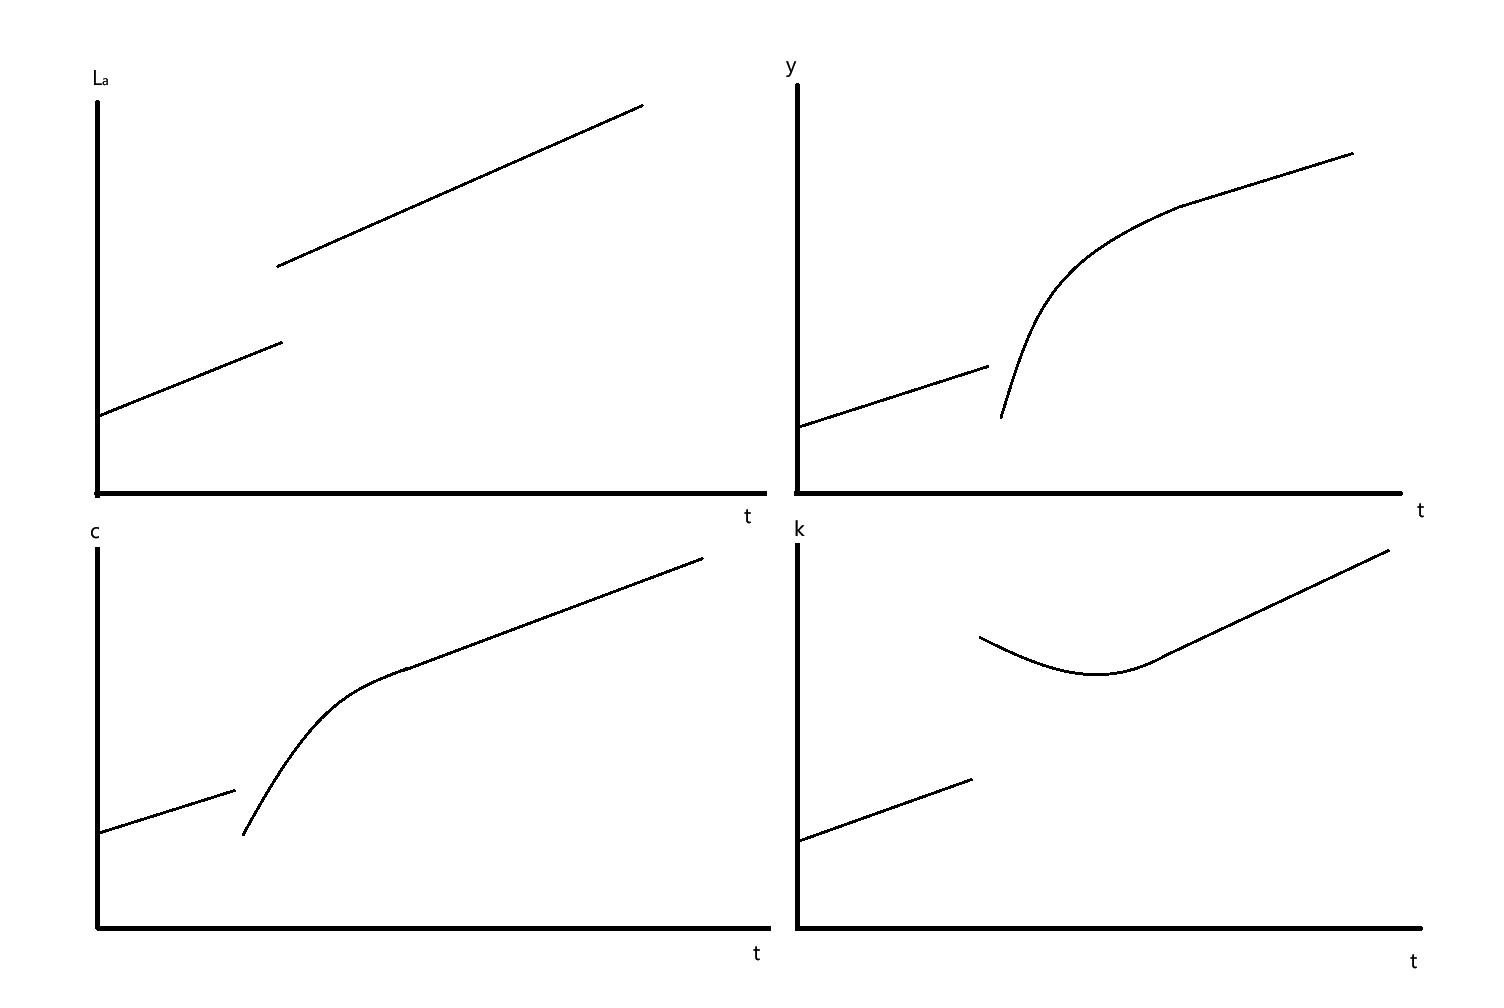
\includegraphics[width=0.8\linewidth]{figure/a1b}
	\end{figure}
	
	\clearpage
	\item \textbf{(8 pts)} 
	\begin{figure}[htbp!]
		\centering
		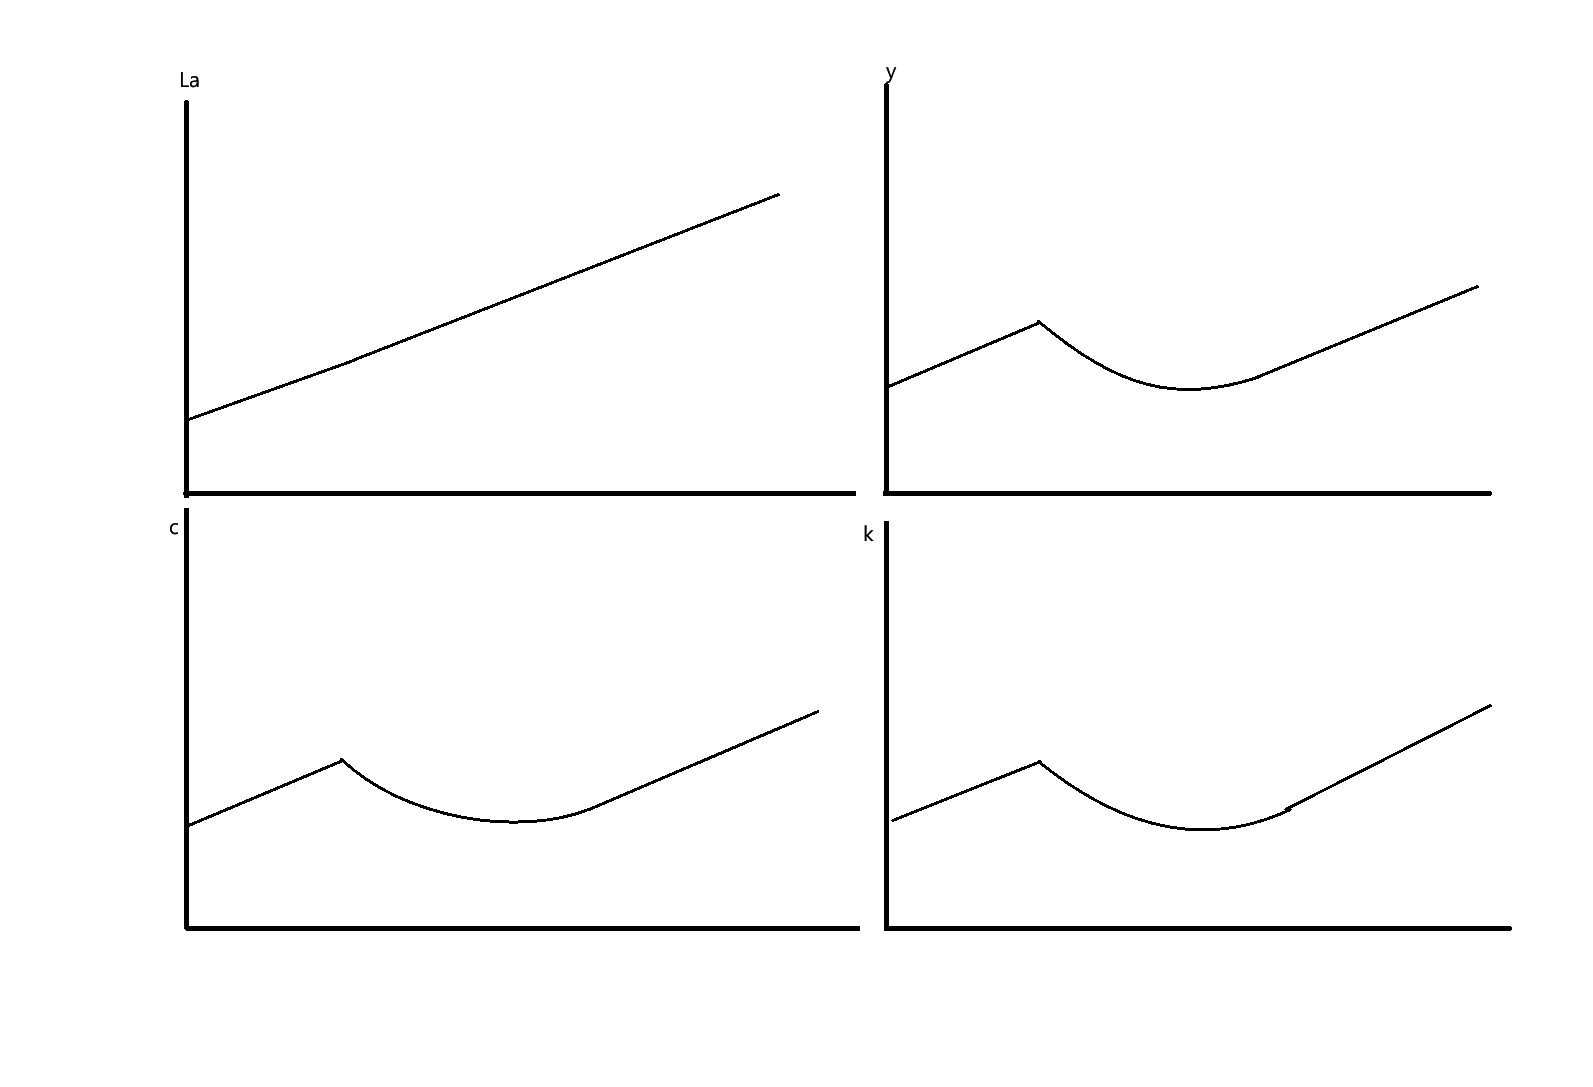
\includegraphics[width=0.85\linewidth]{figure/a1c}
	\end{figure}
	
	\textbf{Grading Scheme}
	For each graph:
	
	\begin{itemize}
		\item 0.25 point: Correctly label both the vertical (y) and horizontal (x) axes.
		\item 0.5 point: Show a constant growth trend (each line should go up over time).
		\item 0.75 point: Illustrate the transition dynamics (the curved adjustment path if applicable).
		\item 0.5 point: Identify the level shift of the balanced growth path (BGP).
	\end{itemize}

	
\end{enumerate}
\clearpage


\item  \textbf{(12 points)} Consider a country in which the following activities occur during 2025: 
\begin{itemize}
	\item A lumber company located in the country pays its workers \$35,000 to harvest 5,000 logs of wood. 
	\item A furniture company purchases the domestically harvested logs for \$40 per log, and pays its workers \$105,000 to produce 100 pieces of furniture, which it sells for \$5,000 each. Of these 100 pieces, 65 are sold to domestic consumers, 30 are sold to the government, and 5 are sold to a international buyer. The furniture company also uses \$50,000 worth of imported hardware. 
\end{itemize}



\begin{enumerate}[label=(\alph*)]
	\item \textbf{(5 pts)} 	What is the GDP of this economy? Calculate it using two of three approach, be sure to show your calculations.
	
	%\clearpage
	
	\item \textbf{(4 pts)} Suppose that in the following year, the quantities of logs harvested and furniture produced remain the same, and wages paid by both companies remain the same, but the price of logs rises to \$55 per log, and the price of a piece of furniture rises to \$5200. The value of the imported hardware remains unchanged. What is the growth rate of real GDP and the growth rate of nominal GDP between the first year and the next? Explain your reasoning
	
	%\vspace{10cm}
	%	
	\item \textbf{(3 pts)} What can we say about the change in the well-being of an average citizen of this country from the first year to the next? Briefly explain
	
\end{enumerate}

\clearpage
\textbf{Solution}
\begin{enumerate}[label=(\alph*)]
	\item \textbf{(5 pts)} 	
	
	Either two of the three:
	
	Expenditure approach:
	
	\[65 \times \$5000 + 30 \times \$5000 + 5 \times \$5000 -\$50000= \$450,000\]
	
	Value-added approach:
	
	From the lumber company:
	\[5000 \times \$40 = \$200,000\]
	
	From the furniture company:
	\[100 \times \$5,000 - 5000 \times \$40  - \$50000= 250,000\]
	
	Together, the GDP = $200000+250000 = 450000$
	
	Income approach:
	\[\$35000 + \$105000 + 5000\times \$40 -35000 + 100 \times \$5000 - 105000 - 5000\times 40 - \$50,000 = \$450,000\]
	
	
	\textbf{*Grading Scheme}
	
	\begin{itemize}
		\item 1 point: show that GDP calculated by the two approaches is identical (0.5 points if they note that the two are not same).
		\item 2 points for each calculation, allocated as follows:
		\begin{itemize}
			\item 0.5 point: Correct formula  
			\item 1 point: use the correct number
			\item 0.5 point: Correct final value  
		\end{itemize}
	\end{itemize}
	
	\clearpage
	\item \textbf{(4 pts)} 
	The growth rate of the real GDP will be zero as in the initial year, because the amount of logs harvested and furniture produced remain the same.
	
	We can update the Expenditure approach:
	
	\[65 \times \$5200 + 30 \times \$5200 + 5 \times \$5200 -\$50000= \$470,000\]
	
	
	The growth rate is then: $470000/450000 - 1 = 0.044444$
	
	\textbf{Grading Scheme}
	
	\begin{itemize}
		\item Real GDP growth rate 
		\begin{itemize}
			\item 1 point: State that real quantities remain unchanged.
			\item 1 point: Show that the growth rate is zero.
		\end{itemize}
		\item Nominal GDP growth rate
		\begin{itemize}
			\item 1 point: Update nominal GDP using new prices.
			\item 1 point: Calculate the growth rate.
		\end{itemize}
	\end{itemize}
	
	%\vspace{10cm}
	%	
	\item \textbf{(3 pts)} There are no changes in the well-being of an average citizen, because the real consumption would be the same as before the change in prices.
	
	\textbf{Grading Scheme}
	\begin{itemize}
		\item 1.5 points: point out well-being should be based on real consumption
		\item 1.5 points: state that there is no change in well-being
	\end{itemize}
	
\end{enumerate}


\clearpage
\item \textbf{(15 points)} Below are figures showing the time path of an economy described by the simple IS curve:
\[
\tilde{Y}_t = \bar{a} - \bar{b}(R_t - \bar{r}),
\]
and the Phillips curve:
\[
\Delta \pi_t = \bar{\nu}\tilde{Y}_t + \bar{o}.
\]

\begin{figure}[htbp!]
	\centering
	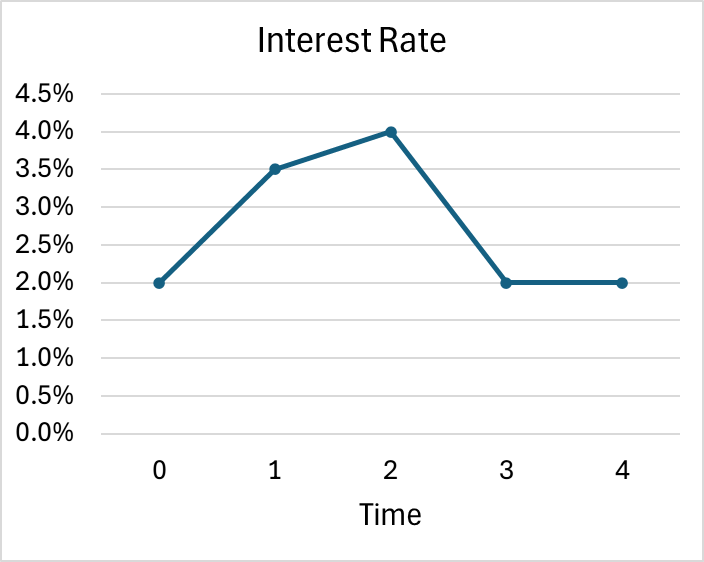
\includegraphics[width=0.4\linewidth]{figure/Q1a}
	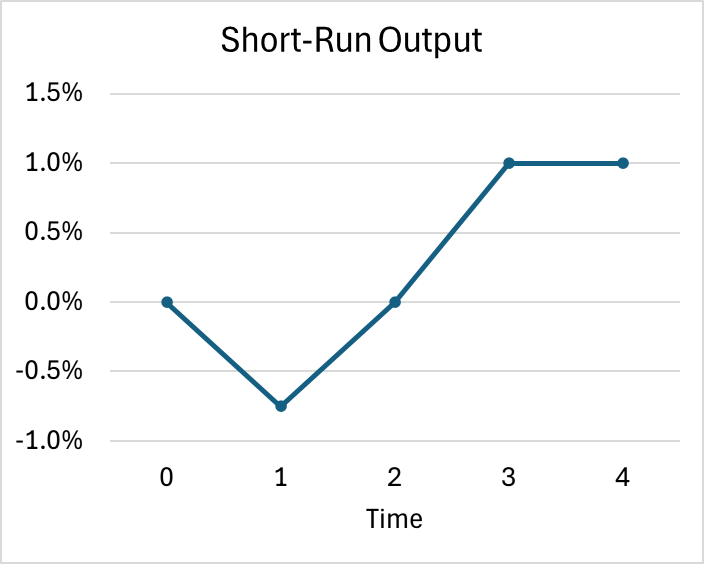
\includegraphics[width=0.4\linewidth]{figure/Q1a2}
	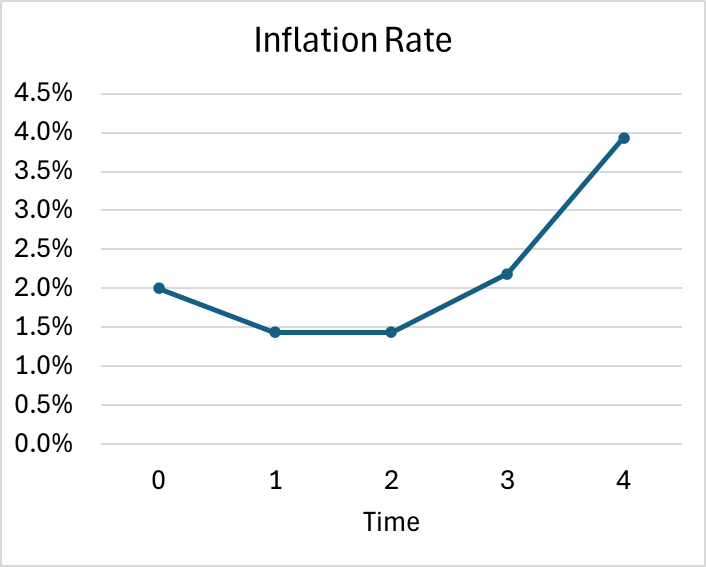
\includegraphics[width=0.4\linewidth]{figure/Q1a3}
\end{figure}

At period 0, the economy is in its steady state. Starting in period 1, the economy undergoes a series of shocks or policy adjustments.

\clearpage
\begin{enumerate}
	\item \textbf{(4 points)} Identify the shocks or policy changes that occur from period 1 through period 4. Justify your reasoning based on the information provided in the figures above (1 to 3 sentences for each period).
	%\clearpage
	\item \textbf{(6 points)} Using an IS/MP diagram along with a Phillips curve diagram, demonstrate how each shock influences the IS curve, the MP curve, and the Phillips curve. Clearly label each graph with the equilibrium points and curves for every period (e.g., use $IS_1$ for the IS curve in period 1 and $E_1$ for its equilibrium, etc.). Alternatively, you may provide a series of graphs to illustrate the changes from one period to the next.
	
%	\vspace*{\fill}
%	\clearpage
	\item \textbf{(3 points)} Explain how the central bank controls the nominal interest rate in the overnight market. Also, discuss why commercial banks (e.g., TD, BoM, CIBC, RBC, etc.) would not borrow or lend at rates different from that set by the Bank of Canada. Provide your explanation in 4–6 sentences.
%	\vspace{8cm}
	\item \textbf{(2 points)} For the MP curve, state the assumption necessary for the central bank to adjust the real interest rate. Explain your answer in 3–5 sentences.
\end{enumerate}


\clearpage
\textbf{Solution}
\begin{enumerate}
	\item \textbf{(4 points)} In period 1, the central bank has rise the interest rate, resulting a fall in $\tilde{Y}$ and $\pi$. 
	
	In period 2, the interest rate continue to rise but the $\tilde{Y}$ return to zero. This can only happen if there is an increase in aggregate demand $\bar{a}$.
	
	In period 3, it is most likely because of a fall in interest rate as we observe the fall in the figure and a rise in $\tilde{Y}$ ($\bar{a}$ could also increase, it is not necessary to obtain the observation 
	
	In period 4, there are no changes in interest rate or $\bar{a}$. As the short-run output is positive, it lead to an increase in the inflation rate. However, we can observe that the the inflation rate increase faster than before. Therefore, there is an positive price shock as well ($\bar{o}$)
	
	%\clearpage
	\item \textbf{(6 points)} 
	
	\begin{figure}[htbp!]
		\centering
		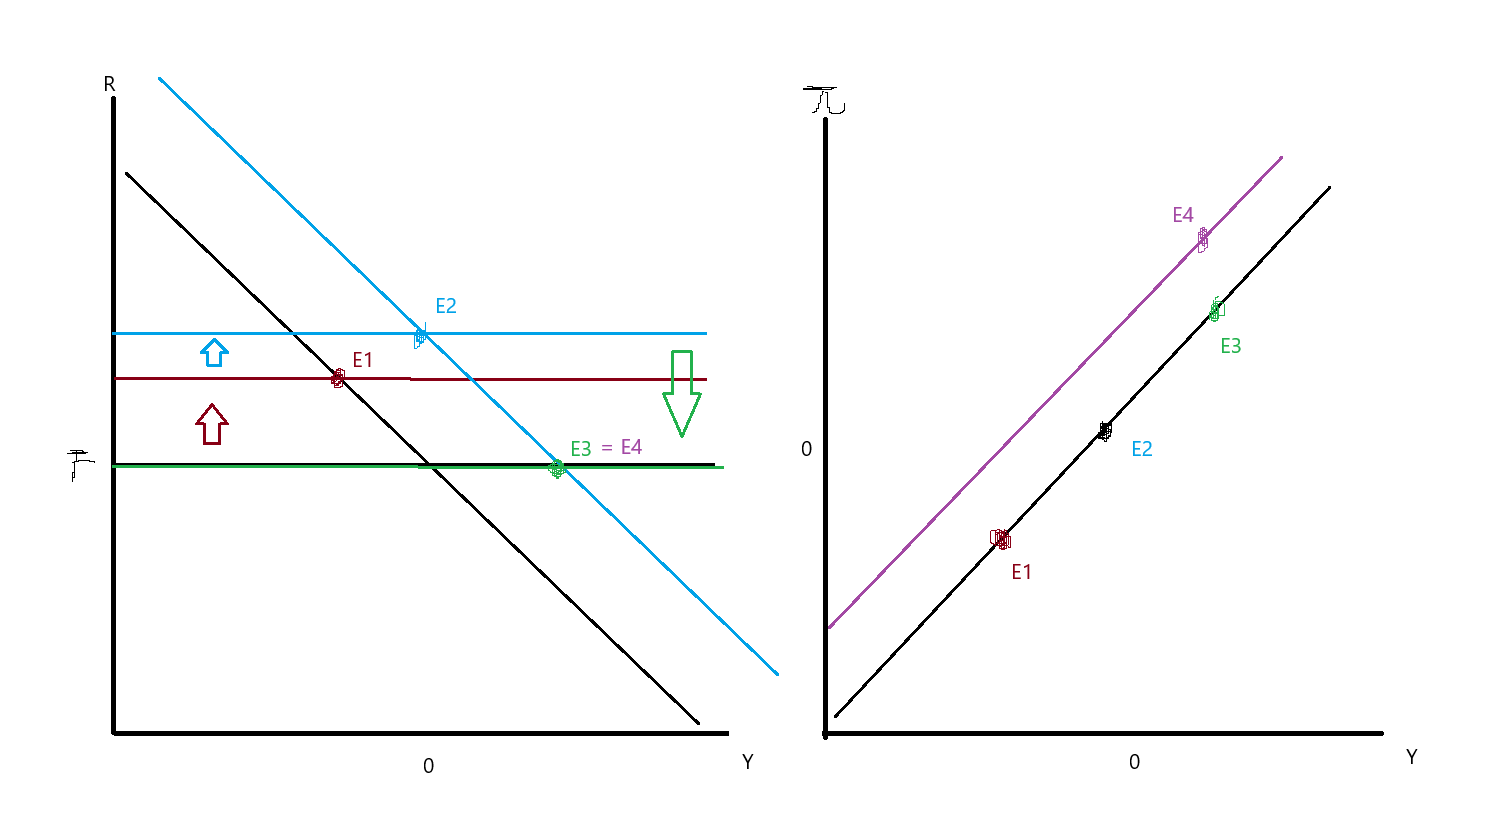
\includegraphics[width=0.9\linewidth]{figure/a2b}
	\end{figure}
	
	
	\vspace*{\fill}
	\clearpage
	\item \textbf{(3 points)} The central bank sets a specific nominal interest rate by acting as both a lender and a borrower in the overnight market, effectively establishing a rate corridor. Because the central bank would lend money at the target rate, no commercial bank would borrow funds above that rate as they can always borrow from the central bank. 	
	 Similarly, since the central bank is willing to accept deposits at that rate, banks would not be able to earn a higher rate by lending to each other, since any surplus funds would instead be channeled into the central bank’s facility. This mechanism ensures that the market interest rate is anchored around the central bank’s target.
	
	
	\item \textbf{(2 points)} For the MP curve, the necessary assumption for the central bank to adjust the real interest rate is that prices/inflation is sticky in the short run. This assumption implies that changes in the nominal interest rate, will translate into adjustments in the real interest rate.
\end{enumerate}





\newpage
%\begin{center}
%	This page is intentionally left blank. Please continue your answer to Question 2 below.
%\end{center}
%\vspace*{\fill}
%\newpage


\item \textbf{(17 points)}   Consider the consumption model discussed in Ch.16, the consumer has the following utility function:
\[U = ln(c) + \beta ln(c')\]
where $c$ is the consumption in the current period, $c'$ is the consumption in the future period and $\beta$ is the discount factor. A consumer begins with assets valued at \(f\) and will hold assets \(f'\) in the future. When these assets roll over to the next period, they generate interest income of \(rf'\), where \(r\) represents the interest rate. In current period, the consumer receive $y$ amount of income. In the future period, the consumer receives $y'$ amount of income. 

The government implements a form of social security. Under this policy, it collects a portion $\tau$ of an individual's current income and returns it, with interest, as a future benefit. Specifically, the consumer pays $\tau y$ to the government in the current period and receives $(1 + r)\tau y$ in the future period, where $\tau$ is the tax rate and $r$ is the interest rate. 
\begin{enumerate}[label=(\alph*)]
	\item \textbf{(2 pts)} 	Setup the budget constraint. Shows the current period budget constraint, future period budget constraint and the lifetime budget constraint.
		
%	\clearpage
	
	\item \textbf{(4 pts)}  Derive the Euler equation and derive the optimal $c$ and $c'$.
	
%	\clearpage
	\item \textbf{(2 pts)} What is the maximum amount the consumer can consume in the current period if they are not allowed to borrow against their social security income (i.e., they cannot use future social security income to repay a loan)? (Note: This borrowing constraint remains in effect in parts (d) through (f).)
	
%	\vspace{6cm}
	
	\item \textbf{(4 pts)} Given that \(\beta = 0.80\), \(f = 0\), \(r = 0.10\), \(y = 550\), \(y' = 100\), and \(\tau = 0.40\), determine whether the consumer is a saver or a borrower.
	
	
%	\clearpage
	\item \textbf{(3 pts)} If the government increases \(\tau\) to 0.6, what is the optimal consumption bundle (i.e., \(c^*\) and \(c^{\prime*}\))?
	
%	\vspace{10cm}
	
	\item \textbf{(2 pts)} In general, can the consumer smooth consumption perfectly with this social security? Explain your answer in 2–5 sentences.
	

\end{enumerate}

\clearpage
\textbf{Solution}
\begin{enumerate}[label=(\alph*)]
	\item 
		Current period budget constraint
		\[c = y +f -f' -\tau y\]
		
		Future period budget constraint
		\[c' = y' +(1+r)f' +(1+r)\tau y\]
		
		Lifetime budget constraint:
		\[c+\frac{c'}{1+r} = \frac{y'}{1+r} +y+f\]
	
	\item 
		The utility function:
		\[\ln\left(y + \frac{y'}{1+r} +f - \frac{c'}{1+r} \right) + \beta\ln(c')\]
		The first order condition w.r.t. c':
		\[\left(\frac{1}{c}\right) \frac{1}{1+r} = \frac{\beta}{c'}\]
		
		Rearrange:
		\[\frac{c'}{c} = \beta \left(1+r\right)\]
		
		Plug the Euler equation back to the budget constraint.
		
		\[c+\frac{ \beta \left(1+r\right) c}{1+r} = y+\frac{y'}{1+r} + f\]
		
		\[c+ \beta  c  = y+\frac{y'}{1+r} + f \implies c = \left(\frac{1}{1+\beta}\right) \left[y+\frac{y'}{1+r} + f\right] \]
		
		, and
		\[c'=  \left(1+r\right) \left(\frac{\beta}{1+\beta}\right) \left[y+\frac{y'}{1+r} + f\right] \]
	
	\clearpage
	\item We can start from how much can one consume in the current period: $c_{max} = \frac{y'}{1+r}-\tau y +y+f$.
	
	Subtract it by the amount of initial wealth and current income, the consumer can borrow only up to $\frac{y'}{1+r}-\tau y$.
	
	%\vspace{8cm}
	\item Plug in the number into the optimal $c$ questions 
	\[c^* = 356.06\]
	Meanwhile, the maximum amount of current consumption allowed is $\frac{100}{1+0.1}- (0.4) 550 +550+0  = 0.4 (550) = 420.9$
	
	Therefore, the consumer would choose to consume $c^* = 356.06$
	
	Based on this, we can calculate if the consumer is saving or borrowing:
	\[c^* = 356.06 < y + f = 550 \]
	
	Therefore, the consumer is consume less than the earning plus initial wealth, which implies the consume is a saver.
	
	\item Increase the $\tau$ to 0.6. It won't change the $c^*$ but it would reduce how much the consumer are allowed to consume under the constraint, which amount to $310.90$.  Since $c^* = 356.06 > 310.9$, the consumer would choose only consume at the maximum amount at 310.9
	
	
	
	\item No, the consumer cannot perfectly smooth consumption under this social security arrangement. Unlike in a perfect financial market, borrowing constraints prevent the consumer from borrowing against future social security income, which means they cannot freely choose their optimal consumption bundle. Part d) and e) are an example of it. The consumer would have to choose the $c_{max}$ instead of the optimal consumption bundle calculated from the utility maximization problem.
	
	
\end{enumerate}



%\newpage
%\begin{center}
%	This page is intentionally left blank. Please continue your answer to Question 3 below.
%\end{center}
%\vspace*{\fill}

\newpage

\item  \textbf{(22 pts)}\label{P4} Suppose the economy begins at a steady state where GDP is at its potential, the real interest rate equals the marginal product of capital at 4 percent, and the inflation rate stands at 3 percent. Moreover, the economy can be described by the following equations:
\begin{itemize}
	\item IS Curve: 
	\[
	\tilde{Y}_t = \frac{1}{1-\bar{x}}\left[\bar{a} - \bar{b}(R_t-\bar{r})\right]
	\]
	\item Phillips Curve: 
	\[
	\pi_{t} = \pi_{t-1} + \bar{\nu}\tilde{Y}_t + \bar{o}
	\]
	
\end{itemize}

\begin{enumerate}[label=(\alph*)]
	\item \textbf{(3 pts)} Suppose the economy experiences a positive aggregate demand shock. To neutralize this shock, what policy measures should the central bank implement? Explain how the policy works in 2–3 sentences, and illustrate your answer using both an IS/MP diagram and a Phillips curve diagram.
%	\clearpage
	
	\item \textbf{(1 pts)} Derive the AD and AS curves using the Simple Monetary Rule:
	\[
	R_t - \bar{r} = \bar{m} \left(\pi_t - \bar{\pi}\right)
	\]
%	\vspace{5cm}
	\item \textbf{(3 pts)} Analyze the effect of a positive aggregate demand shock (assume it to stay for a long period) in an AD/AS diagram, including both the initial impact and the subsequent adjustment (use arrow to present any gradual moment).
%	\clearpage
	\item \textbf{(3 pts)} Now, suppose the central bank aims to sustain positive short-run output. Based on the simple monetary rule, what actions must the central bank take? Illustrate your answer by indicating a shift in the AD or AS curve on the previous graph (you may also redraw the AD/AS diagram here if needed).
%	\clearpage
	\item \textbf{(6 pts}) Show the time path of \(R_t\), \(\tilde{Y}_t\), and \(\pi_t\)  for the analysis outlined in parts (c) through (d).
%	\clearpage
	\item \textbf{(6 pts)} (separate from part c,d,e) Suppose the parameter \(\bar{x}\) increases. How does this change affect the AD or AS curve? For an identical positive price shock, explain how the impact on short-run output would differ. Provide your explanation in 2–4 sentences. In an AD/AS diagram, illustrate this by showing the original curves (labeled \(AD\) and \(AS\)) and the curves after the shock (labeled \(AD'\) and \(AS'\)).
\end{enumerate}

\clearpage
\textbf{Solution}

\begin{enumerate}[label=(\alph*)]
	\item \textbf{(3 pts)} The central bank would have to increase the interest rate to neutralize the shock. By increasing the interest rate, firms would have less incentive to invest which lead to a decrease in investment. Therefore, it would lower the short-run output, which shift the IS curve to the left.
	
	
	\begin{figure}[htbp!]
		\centering
		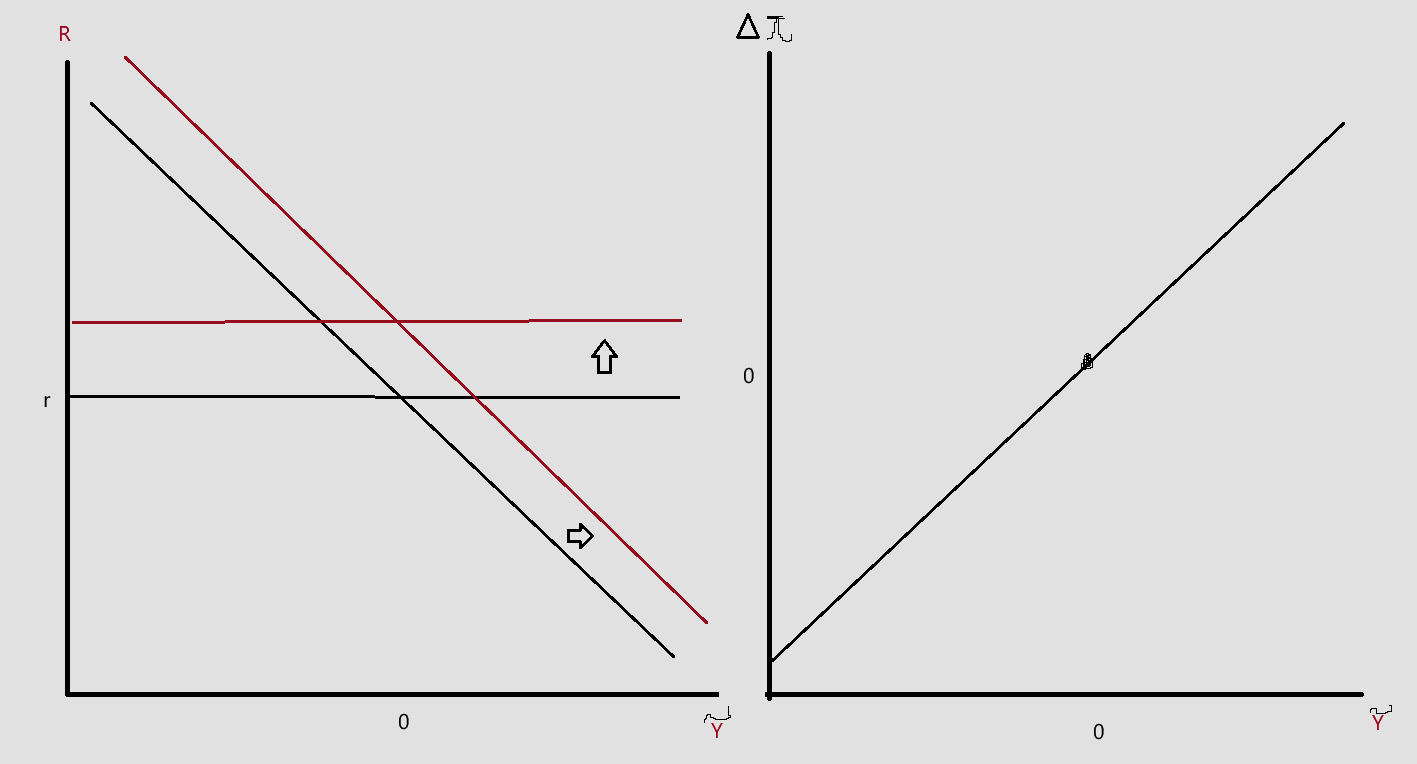
\includegraphics[width=0.7\linewidth]{figure/Q5a}
	\end{figure}
	
	
	%	\clearpage
	
	\item \textbf{(1 pts)} Substitute the Simple Monetary Rule into the IS equation to express the short run output in terms of inflation:
	\[
	\tilde{Y}_t = \frac{1}{1-\bar{x}}\left[\bar{a} - \bar{b}\left(\bar{m}(\pi_t-\bar{\pi})\right)\right].
	\]
	This equation represents the Aggregate Demand (AD) curve in the \((\pi,\tilde{Y})\) space. The Aggregate Supply (AS) curve is given by the Phillips curve:
	\[
	\pi_{t+1} = \pi_t + \bar{\nu}\tilde{Y}_t + \bar{o}.
	\]
	
	\clearpage
	%	\vspace{5cm}
	\item \textbf{(3 pts)} Analyze the effect of a positive aggregate demand shock (assume it to stay for a long period) in an AD/AS diagram, including both the initial impact and the subsequent adjustment (use arrow to present any gradual moment).
	
	\begin{figure}[htbp!]
		\centering
		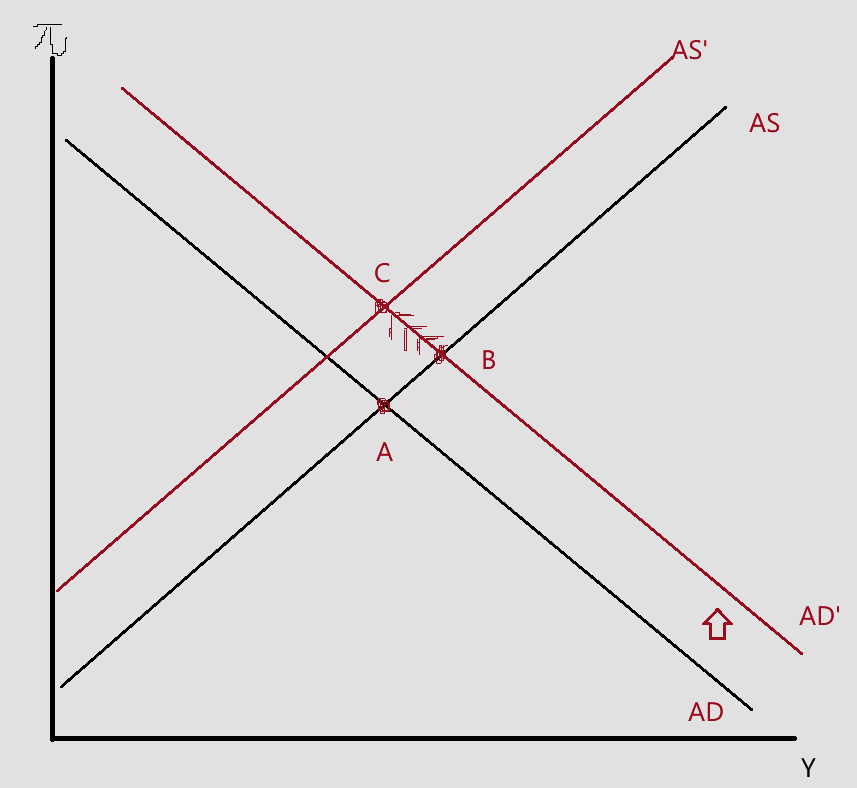
\includegraphics[width=0.7\linewidth]{figure/Q5c}
	\end{figure}
	
	The equilibrium moves from point A to B then gradually to point C.
	
	\clearpage
	\item \textbf{(3 pts)} 
	To sustain positive short‑run output, the central bank must keep shifting the AD curve upward as the AS curve adjusts. In practice, this means raising its inflation target whenever inflation expectations (in the AS curve) rise. On the graph, an increase in the expected inflation rate $\bar\pi$ drives the AD curve higher. Moving the equilibrium to point D.
	
	\begin{figure}[htbp!]
		\centering
		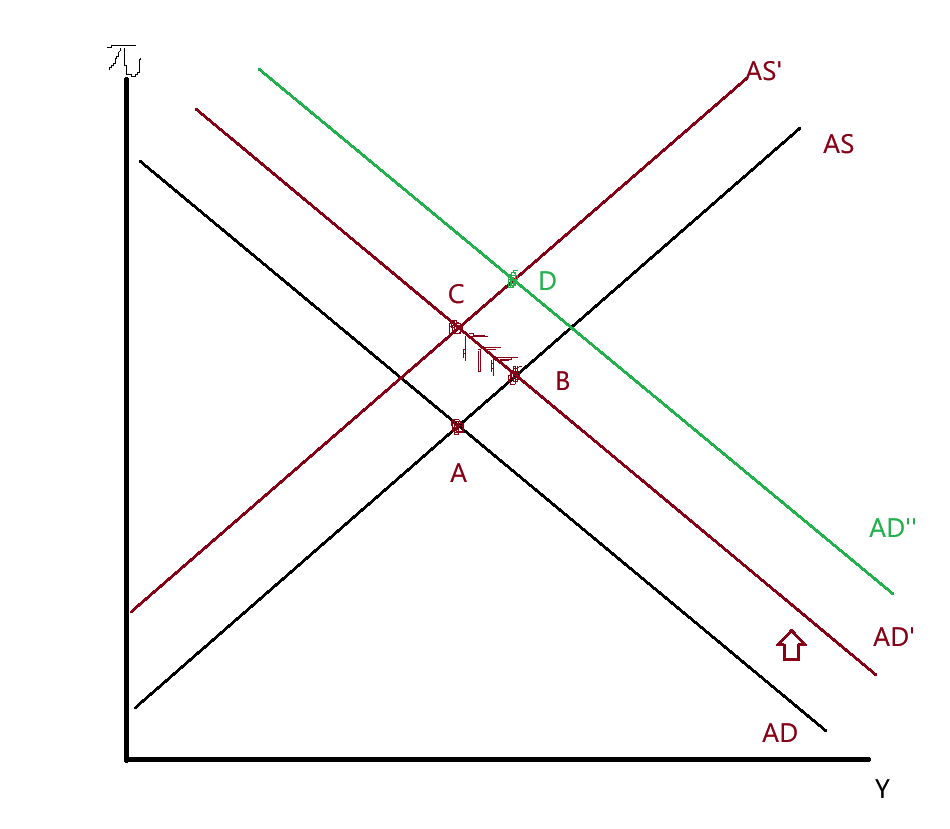
\includegraphics[width=0.7\linewidth]{figure/Q5d}
	\end{figure}
	
	\clearpage
	
	
	\item \textbf{(6 pts}) Show the time path of \(R_t\), \(\tilde{Y}_t\), and \(\pi_t\)  for the analysis outlined in parts (c) through (d).
	
	
	\begin{figure}[htbp!]
		\centering
		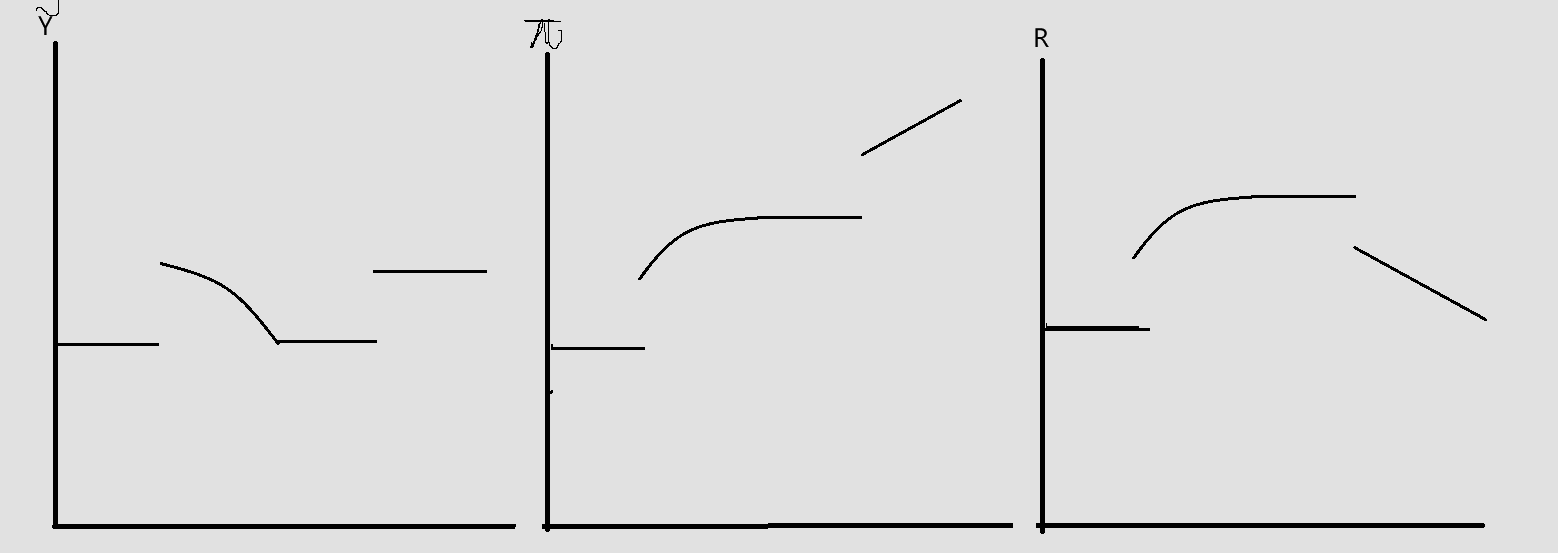
\includegraphics[width=0.7\linewidth]{figure/Q5e}
	\end{figure}
	
	*some students would probably just go from point A to B then to D (instead of to C first). Since the question isn't very clear on that, you can be easy on this.
	
	\clearpage
	\item \textbf{(6 pts)} 
	
	When $\bar{x}$ increases, it would make the AD curve flatter. It would rotate counterclockwise. The AS would remain unchanged when $\bar{x}$ increases.
	
	
	The economy will now become more sensitive to any changes in the interest rate. So, given the same price shocks, the economy with a higher $\bar{x}$ will response more to the same changes in the real interest rate as the central combat the inflation. As a results, a smaller increase in interest rate would lead a larger fall in the short-run output.
	
	
	\begin{figure}[htbp!]
		\centering
		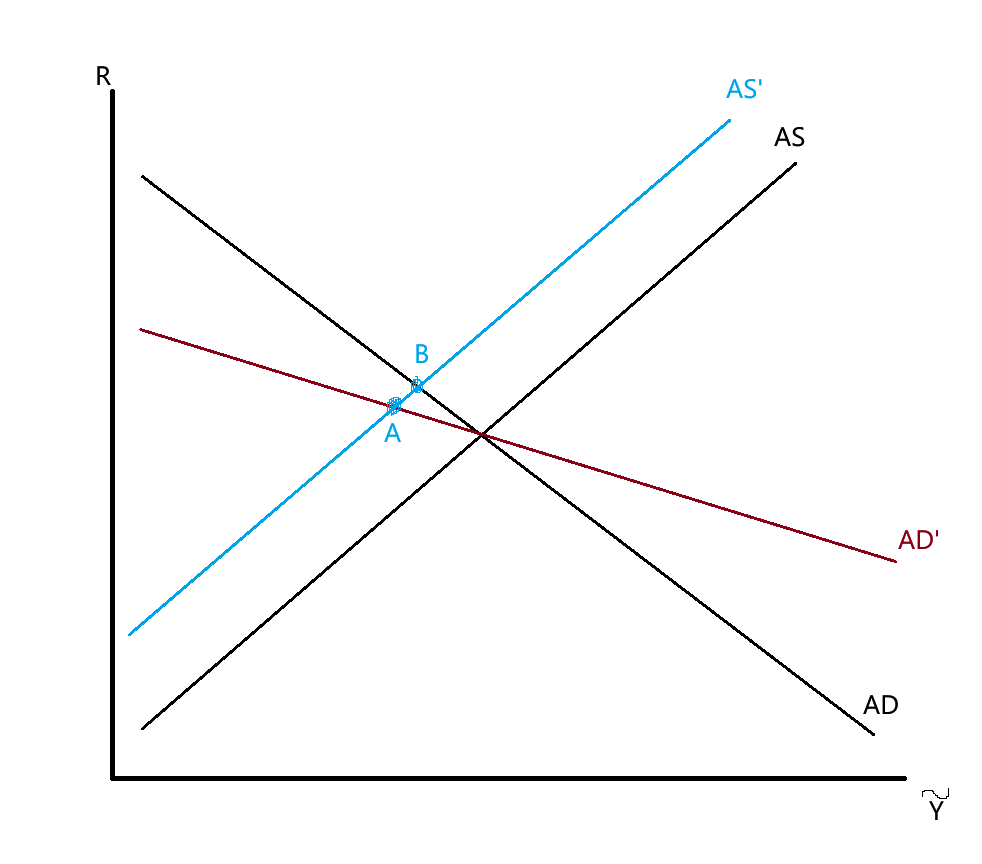
\includegraphics[width=0.7\linewidth]{figure/Q5f}
	\end{figure}
	As seen in the graph, the central bank would move the economy to point A instead of point B if the $\bar{x}$ is higher. Also, we observe that the interest rate increase more in the case of B, since the central bank need to increase the interest rate further to induce a recession.
\end{enumerate}

%\newpage
%\begin{center}
%	This page is intentionally left blank. Please continue your answer to Question 4 below.
%\end{center}
%\vspace*{\fill}

\newpage

\item  \textbf{(11 pts)}  Consider a labour market divided into two groups: old (\( o \)) and young (\( y \)). Each group has its own separation rate (\( \bar{s}_y \) and \( \bar{s}_o \)) and job-finding rate (\( \bar{f}_y \) and \( \bar{f}_o \)). Let \( U_y \) and \( U_o \) represent the number of unemployed individuals in each group, and \( E_y \) and \( E_o \) represent the employed individuals. The total labour force for each group is given by \( L_y = U_y + E_y \) and \( L_o = U_o + E_o \). The evolution of unemployment over time is described by the equations:

\[
\Delta U_{t+1,y} = \bar{s}_y E_{t,y} - \bar{f}_y U_{t,y}
\]
\[
\Delta U_{t+1,o} = \bar{s}_o E_{t,o} - \bar{f}_o U_{t,o}
\]

\begin{enumerate}[label=(\alph*)]
	\item \textbf{(1 pts)} Define the total labour force and the total unemployment rate using the \textit{variables} provided in the question.
	%\vspace{5cm}
	%\clearpage
	\item \textbf{(1 pts)} Determine the equation for the evolution of total unemployment (the young and old group together) over time.
	%\clearpage
	\item \textbf{(3 pts)} Solve for the steady-state unemployment rate for each group.
	%\clearpage
	\item \textbf{(3 pts)} Solve for the steady-state unemployment rate for the economy as a whole as a function of $u_y$, $u_o$, $L_y$ and $L_o$.
	%\clearpage
	\item \textbf{(3 pts)} Data shows that younger workers typically have a higher job separation rate (\( \bar{s} \)) and a lower job finding rate (\( \bar{f} \)) compared to older workers. Following World War II, the baby boom led to a large cohort entering the workforce as young workers 20 years later. How would this demographic shift impact the unemployment rate for each group and the economy as a whole  in the steady state? Explain using the results you have above.
\end{enumerate}

\clearpage
\textbf{Sol'n}
\begin{enumerate}[label=(\alph*)]
	\item \[L=L_y + L_o \text{ Or }= U_y+E_y+U_o+E_o\]
	\[u = \frac{U_y+U_o}{L_y+L_o}\]
	\item \[\Delta U_{t+1,m} + \Delta U_{t+1,f} = \bar{s}_y E_{t,m} - \bar{f}_y U_{t,m} + \bar{s}_o E_{t,f} - \bar{f}_o U_{t,f}\]
	\item 
	Set the changes in $U$ to zero and plug in $L_{t,m}=E_{t,m}+U_{t,m}$ and $L_{t,f}=E_{t,f}+U_{t,f}$
	\[\bar{s}_y E_{t,m} - \bar{f}_y U_{t,m} = 0 \implies \bar{s}_y (L_y - U_y) - \bar{f}_y U_{t,m} =0 \]
	\[\bar{s}_o E_{t,f} - \bar{f}_o U_{t,f} = 0 \implies \bar{s}_o (L_o - U_o) - \bar{f}_o U_{t,f} =0 \]
	Rearrange both equations:
	\[\frac{\bar{s}_y L_y}{\bar{s}_y+\bar{f}_y} =  U_{y} \text{  and  } \frac{\bar{s}_o L_o}{\bar{s}_o+\bar{f}_o} =  U_{o} \]
	Divide both equation by their respective size of labour force to get the unemployment rate:
	\[u_{y} = \frac{\bar{s}_y}{\bar{s}_y+\bar{f}_y}  \text{  and  } u_{o} = \frac{\bar{s}_o }{\bar{s}_o+\bar{f}_o}   \]
	\item \[\frac{U_o + U_y}{L_o+L_y} = \frac{u_oL_o + u_yL_y}{L_o+L_y} = \frac{L_o}{L_o+L_y} u_o + \frac{L_y}{L_o+L_y}u_y\]
	*The equation shows the total unemployment rate is just the weighted average of the unemployment rate.
	\item Since younger workers have a higher job separation rate (\( \bar{s} \)) and a lower job finding rate (\( \bar{f} \)) compared to older workers, the unemployment rate $u_y$ is higher than $u_o$. Therefore, the unemployment are would be higher due to this demographic shift.
\end{enumerate}


\newpage
\item \textbf{(5 points) } Government budget constraint
\begin{enumerate}
	\item	\textbf{(2 point)} Write down and explain the government budget constraint for a single period, identifying all potential sources of financing.
	\vspace{8cm}
	\item	\textbf{(3 point)} If the government announces a tax cut, what are three different approaches to balance the resulting fiscal constraint? Explain each approach in 1–2 sentences.
	%Describe the potential trade-offs that may result from excessive reliance on each source of financing.
%	\clearpage
%	\item \textbf{(2 points)} An aging population and a declining working age population to retiree ratio can pose challenges for the economy in the future. Explain this issue in the context of government budget deficit?
	

	
%	
%	As the population ages, there tends to be a higher demand for government-funded social welfare programs such as pensions, healthcare, and eldercare. This increased demand for services places a strain on government budgets, as more funds are required to support the growing number of retirees. Also, it means that there are fewer people contributing to tax revenues compared to those relying on government benefits.  More importantly, as the population age, the rise in the demand for healthcare is predicted to be the main driver to higher budget deficit.
\end{enumerate}

\clearpage
	\textbf{Soln}
\begin{enumerate}
	\item	\textbf{(2 point)} \[G_t + (1+i)B_t = T_t + B_{t+1} + \Delta M_{t+1}\]
	
	\item	\textbf{(3 point)} Taxes: distort labour decisions, slow long-run growth, politically unpopular since current generation pays in a highly visible manner.
	
	Borrowing: intergenerational wealth transfers, crowding out private	investment, increased risk of default
	
	Seigniorage: hyperinflation and the inflationary tax (with associated moral	hazard issues)
	
\end{enumerate}




%\newpage
%\item  \textbf{(20 pts)}\label{P7} 
%\begin{enumerate}[label=(\alph*)]
%	\item \textbf{(5  pts)} 
%\end{enumerate}
%
%\newpage
%\item  \textbf{(20 pts)}\label{P8} 
%\begin{enumerate}[label=(\alph*)]
%	\item \textbf{(5  pts)} 
%\end{enumerate}
%
%\newpage
%\item  \textbf{(20 pts)}\label{P9} 
%\begin{enumerate}[label=(\alph*)]
%	\item \textbf{(5  pts)} 
%\end{enumerate}
%
%\newpage
%\item  \textbf{(20 pts)}\label{P10} 
%\begin{enumerate}[label=(\alph*)]
%	\item \textbf{(5  pts)} 
%\end{enumerate}

\newpage
\begin{center}
	This page is intentionally left blank. Please continue your answer below.
\end{center}
\vspace*{\fill}

%\newpage
%\begin{center}
%	This page is intentionally left blank. Please continue your answer below.
%\end{center}
%\vspace*{\fill}

\centering{-- The End -- }
\end{enumerate}
  \end{document}
